\documentclass[]{article}
\usepackage{lmodern}
\usepackage{amssymb,amsmath}
\usepackage{ifxetex,ifluatex}
\usepackage{fixltx2e} % provides \textsubscript
\ifnum 0\ifxetex 1\fi\ifluatex 1\fi=0 % if pdftex
  \usepackage[T1]{fontenc}
  \usepackage[utf8]{inputenc}
\else % if luatex or xelatex
  \ifxetex
    \usepackage{mathspec}
  \else
    \usepackage{fontspec}
  \fi
  \defaultfontfeatures{Ligatures=TeX,Scale=MatchLowercase}
\fi
% use upquote if available, for straight quotes in verbatim environments
\IfFileExists{upquote.sty}{\usepackage{upquote}}{}
% use microtype if available
\IfFileExists{microtype.sty}{%
\usepackage{microtype}
\UseMicrotypeSet[protrusion]{basicmath} % disable protrusion for tt fonts
}{}
\usepackage[margin=1in]{geometry}
\usepackage{hyperref}
\hypersetup{unicode=true,
            pdftitle={206 HW 5},
            pdfauthor={Joslyn Fritz},
            pdfborder={0 0 0},
            breaklinks=true}
\urlstyle{same}  % don't use monospace font for urls
\usepackage{graphicx,grffile}
\makeatletter
\def\maxwidth{\ifdim\Gin@nat@width>\linewidth\linewidth\else\Gin@nat@width\fi}
\def\maxheight{\ifdim\Gin@nat@height>\textheight\textheight\else\Gin@nat@height\fi}
\makeatother
% Scale images if necessary, so that they will not overflow the page
% margins by default, and it is still possible to overwrite the defaults
% using explicit options in \includegraphics[width, height, ...]{}
\setkeys{Gin}{width=\maxwidth,height=\maxheight,keepaspectratio}
\IfFileExists{parskip.sty}{%
\usepackage{parskip}
}{% else
\setlength{\parindent}{0pt}
\setlength{\parskip}{6pt plus 2pt minus 1pt}
}
\setlength{\emergencystretch}{3em}  % prevent overfull lines
\providecommand{\tightlist}{%
  \setlength{\itemsep}{0pt}\setlength{\parskip}{0pt}}
\setcounter{secnumdepth}{0}
% Redefines (sub)paragraphs to behave more like sections
\ifx\paragraph\undefined\else
\let\oldparagraph\paragraph
\renewcommand{\paragraph}[1]{\oldparagraph{#1}\mbox{}}
\fi
\ifx\subparagraph\undefined\else
\let\oldsubparagraph\subparagraph
\renewcommand{\subparagraph}[1]{\oldsubparagraph{#1}\mbox{}}
\fi

%%% Use protect on footnotes to avoid problems with footnotes in titles
\let\rmarkdownfootnote\footnote%
\def\footnote{\protect\rmarkdownfootnote}

%%% Change title format to be more compact
\usepackage{titling}

% Create subtitle command for use in maketitle
\newcommand{\subtitle}[1]{
  \posttitle{
    \begin{center}\large#1\end{center}
    }
}

\setlength{\droptitle}{-2em}

  \title{206 HW 5}
    \pretitle{\vspace{\droptitle}\centering\huge}
  \posttitle{\par}
    \author{Joslyn Fritz}
    \preauthor{\centering\large\emph}
  \postauthor{\par}
      \predate{\centering\large\emph}
  \postdate{\par}
    \date{11/28/2018}

\usepackage{booktabs}
\usepackage{longtable}
\usepackage{array}
\usepackage{multirow}
\usepackage[table]{xcolor}
\usepackage{wrapfig}
\usepackage{float}
\usepackage{colortbl}
\usepackage{pdflscape}
\usepackage{tabu}
\usepackage{threeparttable}
\usepackage{threeparttablex}
\usepackage[normalem]{ulem}
\usepackage{makecell}

\begin{document}
\maketitle

\paragraph{1. Compare trends in graduate enrollment
(1967-2015)}\label{compare-trends-in-graduate-enrollment-1967-2015}

Male: t(47) = 16.61, p \textless{} 0.001. Reject the null. Correlation =
0.92, which is a strong positive correlation.

Year significantly predicts male graduate school enrollment (\emph{b} =
-17112153, t(47) = 16.61, \emph{p} \textless{} 0.001) with a strong
positive correlation between the two (Pearson's \emph{r} = 0.92). The
overall model (Total gradute male enrollment = 9060(year) - 17112153)
explains a significant amount of variance in male enrollment (F(1,47) =
276, \emph{p} \textless{} 0.001, R\textsuperscript{2} = 0.85).

Female: t(47) = 51.66, p \textless{} 0.001. Reject the null. Correlation
= 0.99, which is a strong positive correlation.

Year significantly predicts female graduate school enrollment (\emph{b}
= -17112153, t(47) = 16.61, \emph{p} \textless{} 0.001) with a strong
positive correlation between the two (Pearson's \emph{r} = 0.92). The
overall model (Total gradute female enrollment = 30126(year) - 58955502)
explains a significant amount of variance in male enrollment (F(1,47) =
2669, \emph{p} \textless{} 0.001, R\textsuperscript{2} = 0.98).

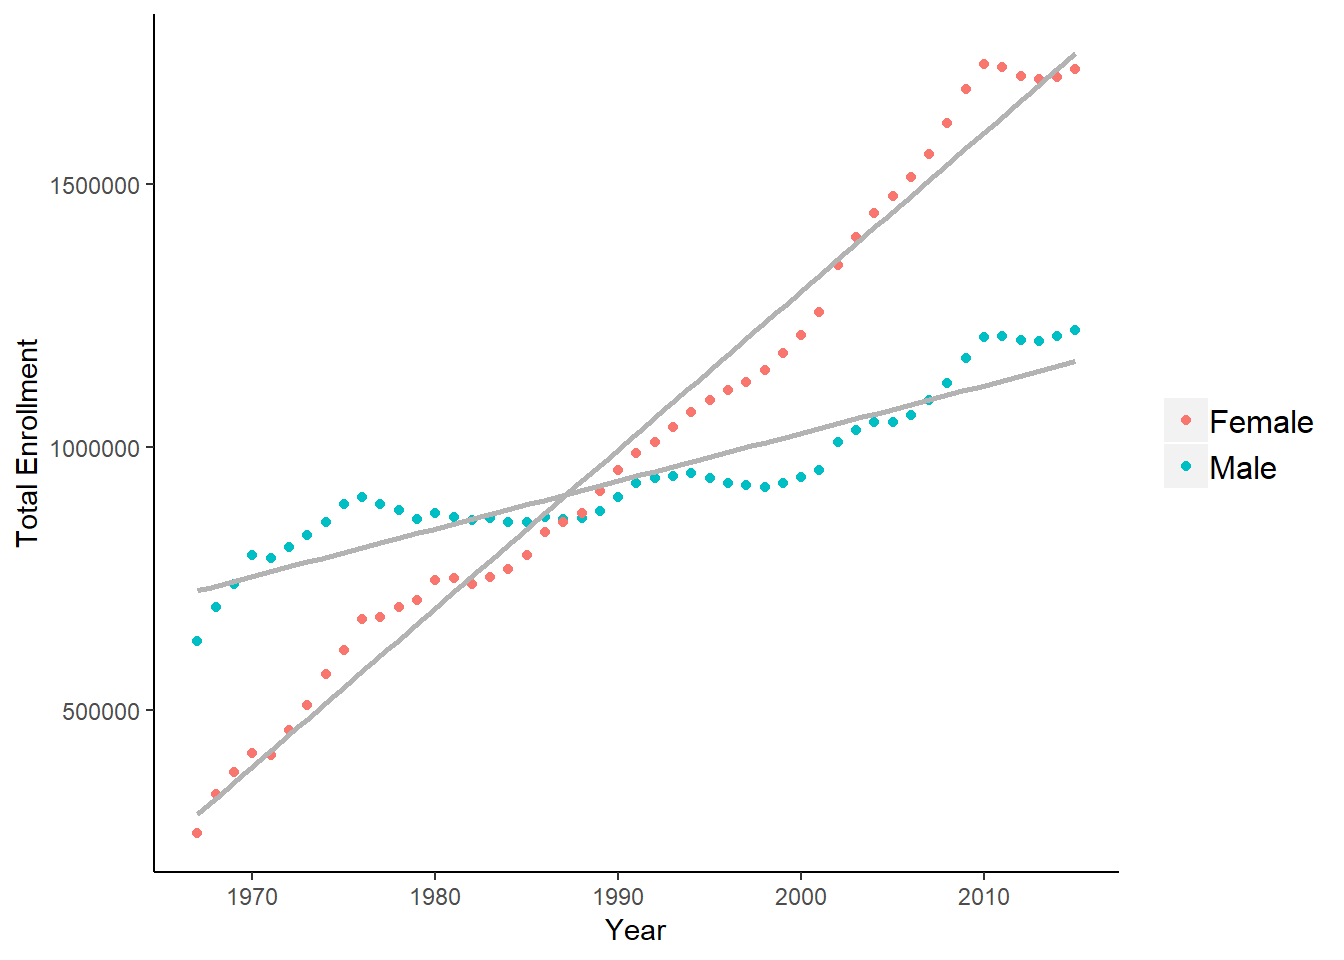
\includegraphics{206_HW_5_files/figure-latex/unnamed-chunk-5-1.pdf}

\paragraph{2. Shifts in Phd recipients by field of study (1985, 2000,
2015)}\label{shifts-in-phd-recipients-by-field-of-study-1985-2000-2015}

number of female phd recipients per field differed significantly between
1985 (n = ) and 2000 (n = ) and 2015 (n =) (\(\chi^2\)\{6\} =
\ldots{}.., p \textless{} 0.001). Notably, \ldots{}.

\begin{table}

\caption{\label{tab:unnamed-chunk-7}**Table 1. Proportions of female recipients who earned a Phd in 1985, 2000 and 2015.**}
\centering
\begin{tabular}[t]{>{\bfseries\raggedright\arraybackslash}p{12em}|>{\raggedleft\arraybackslash}p{8em}|>{\raggedleft\arraybackslash}p{8em}|>{\raggedleft\arraybackslash}p{8em}}
\hline
  & 1985 & 2000 & 2015\\
\hline
Education & 0.31 & 0.37 & 0.31\\
\hline
Engineering & 0.06 & 0.25 & 0.69\\
\hline
Humanities \& Art & 0.20 & 0.39 & 0.41\\
\hline
Physical Earth Sciences & 0.16 & 0.29 & 0.56\\
\hline
\end{tabular}
\end{table}

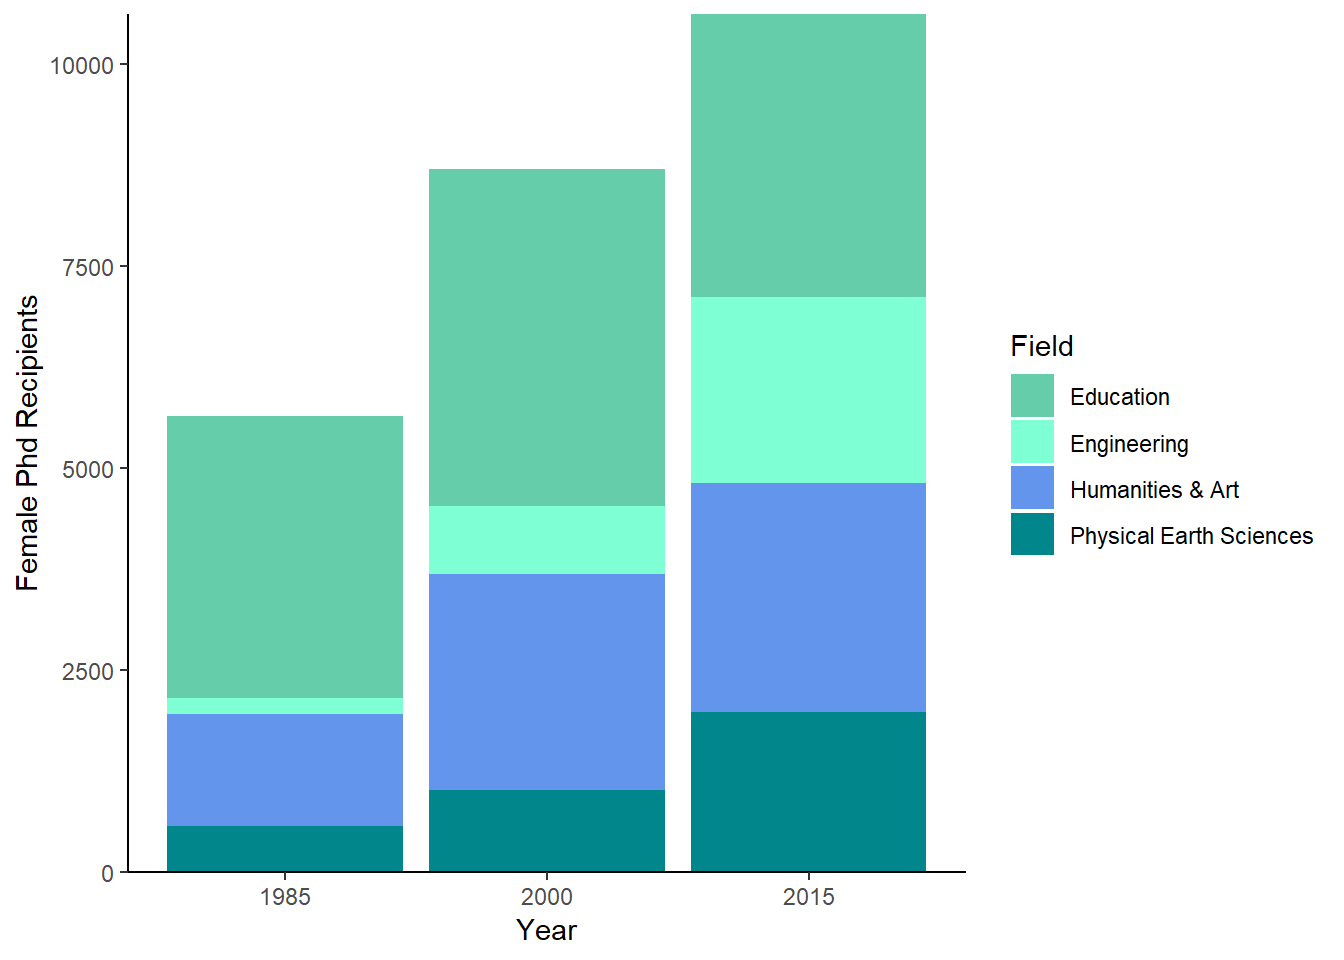
\includegraphics{206_HW_5_files/figure-latex/unnamed-chunk-7-1.pdf}

\paragraph{3. Male and female salaries for starting postdoc and other
positions
(2015)}\label{male-and-female-salaries-for-starting-postdoc-and-other-positions-2015}

Does median salary differ significantly between male and female starting
postdoc positions? Does median salary differ significantly between male
and female PhD recipients in non-postdoc employment positions?

\begin{center}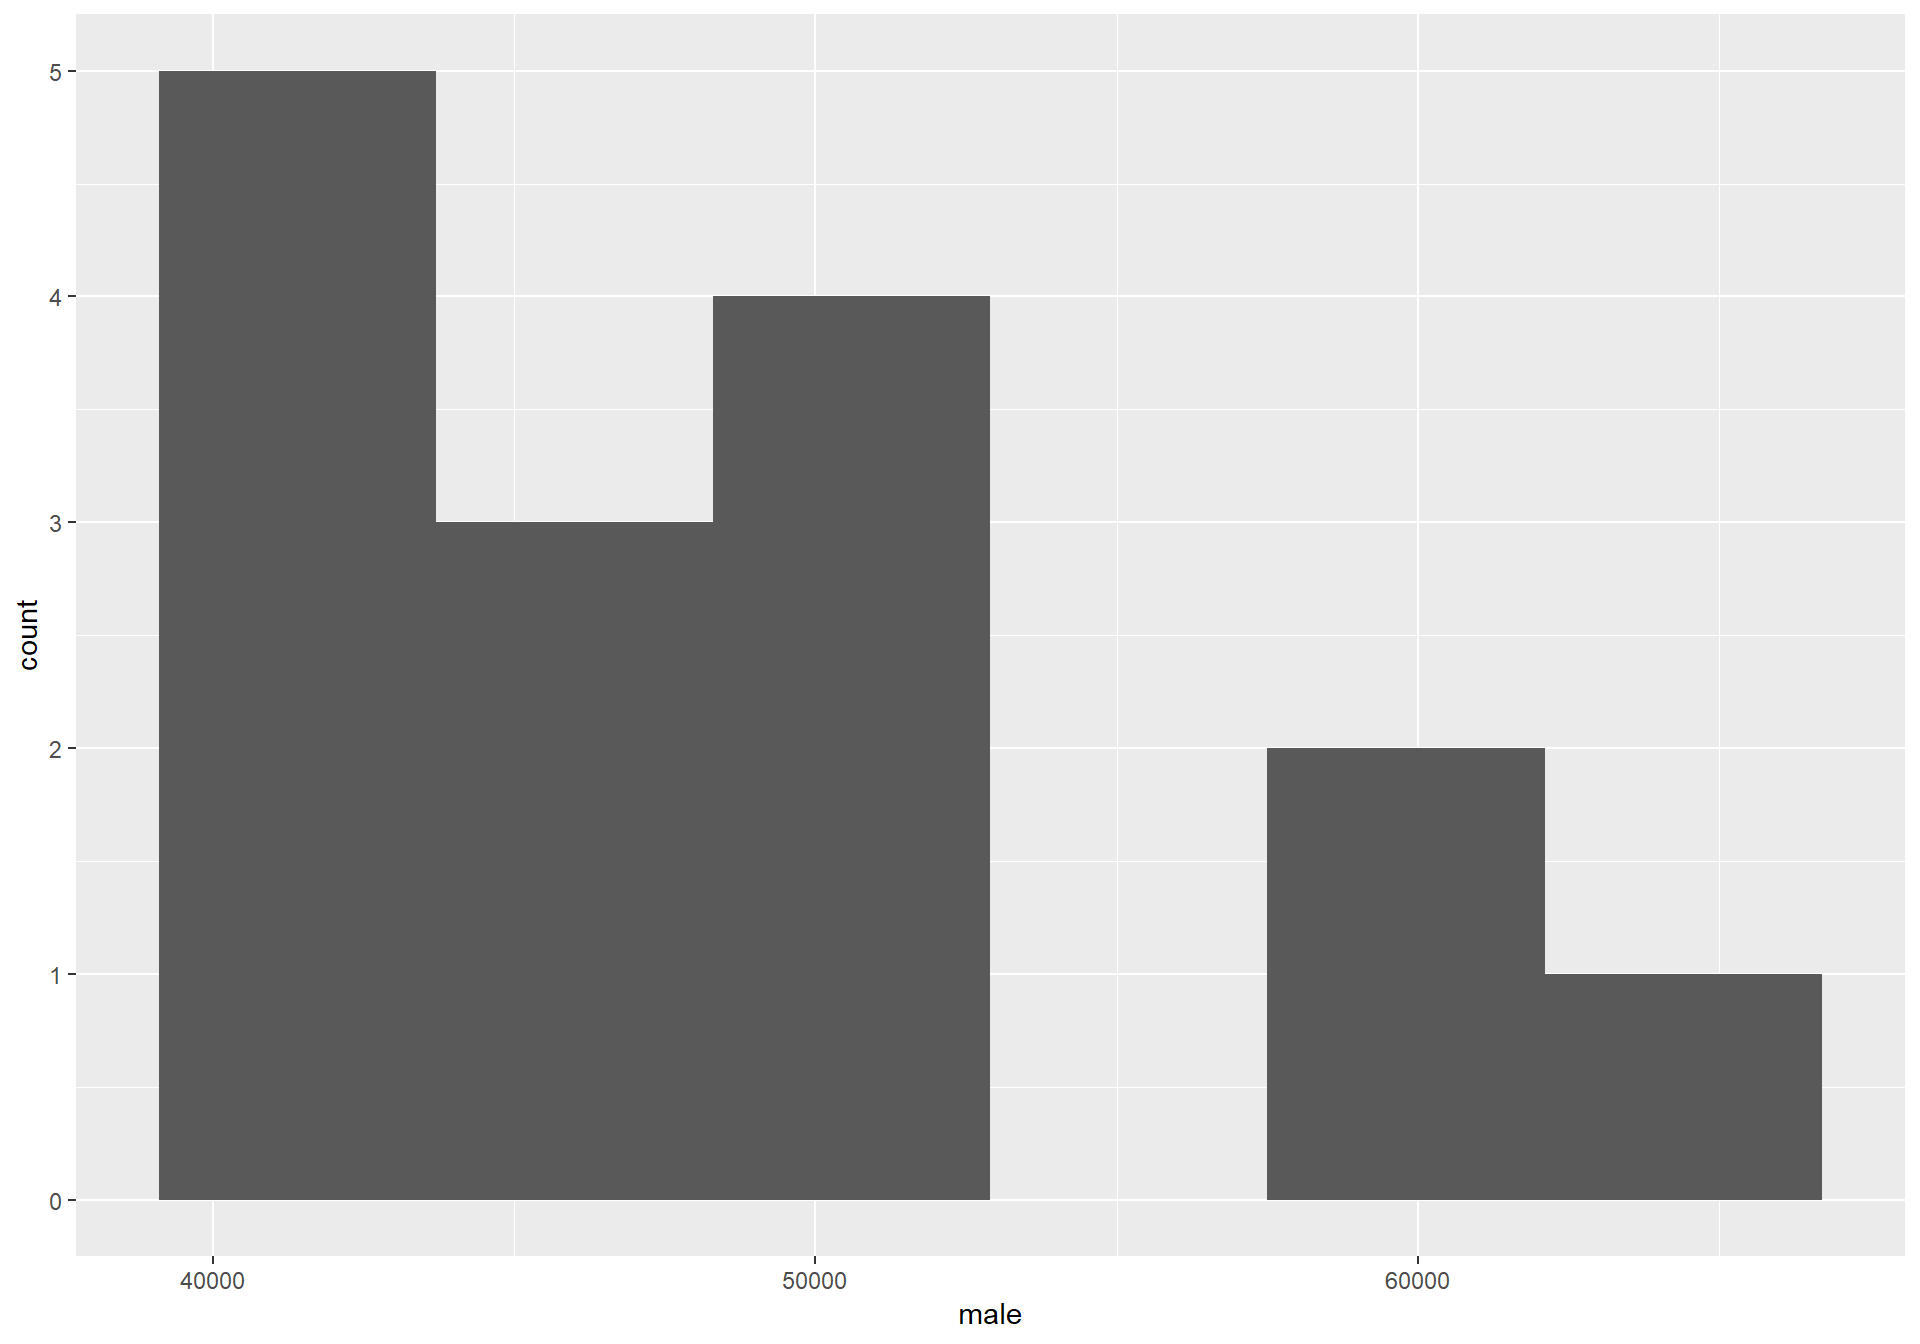
\includegraphics{206_HW_5_files/figure-latex/unnamed-chunk-8-1} \end{center}

\begin{center}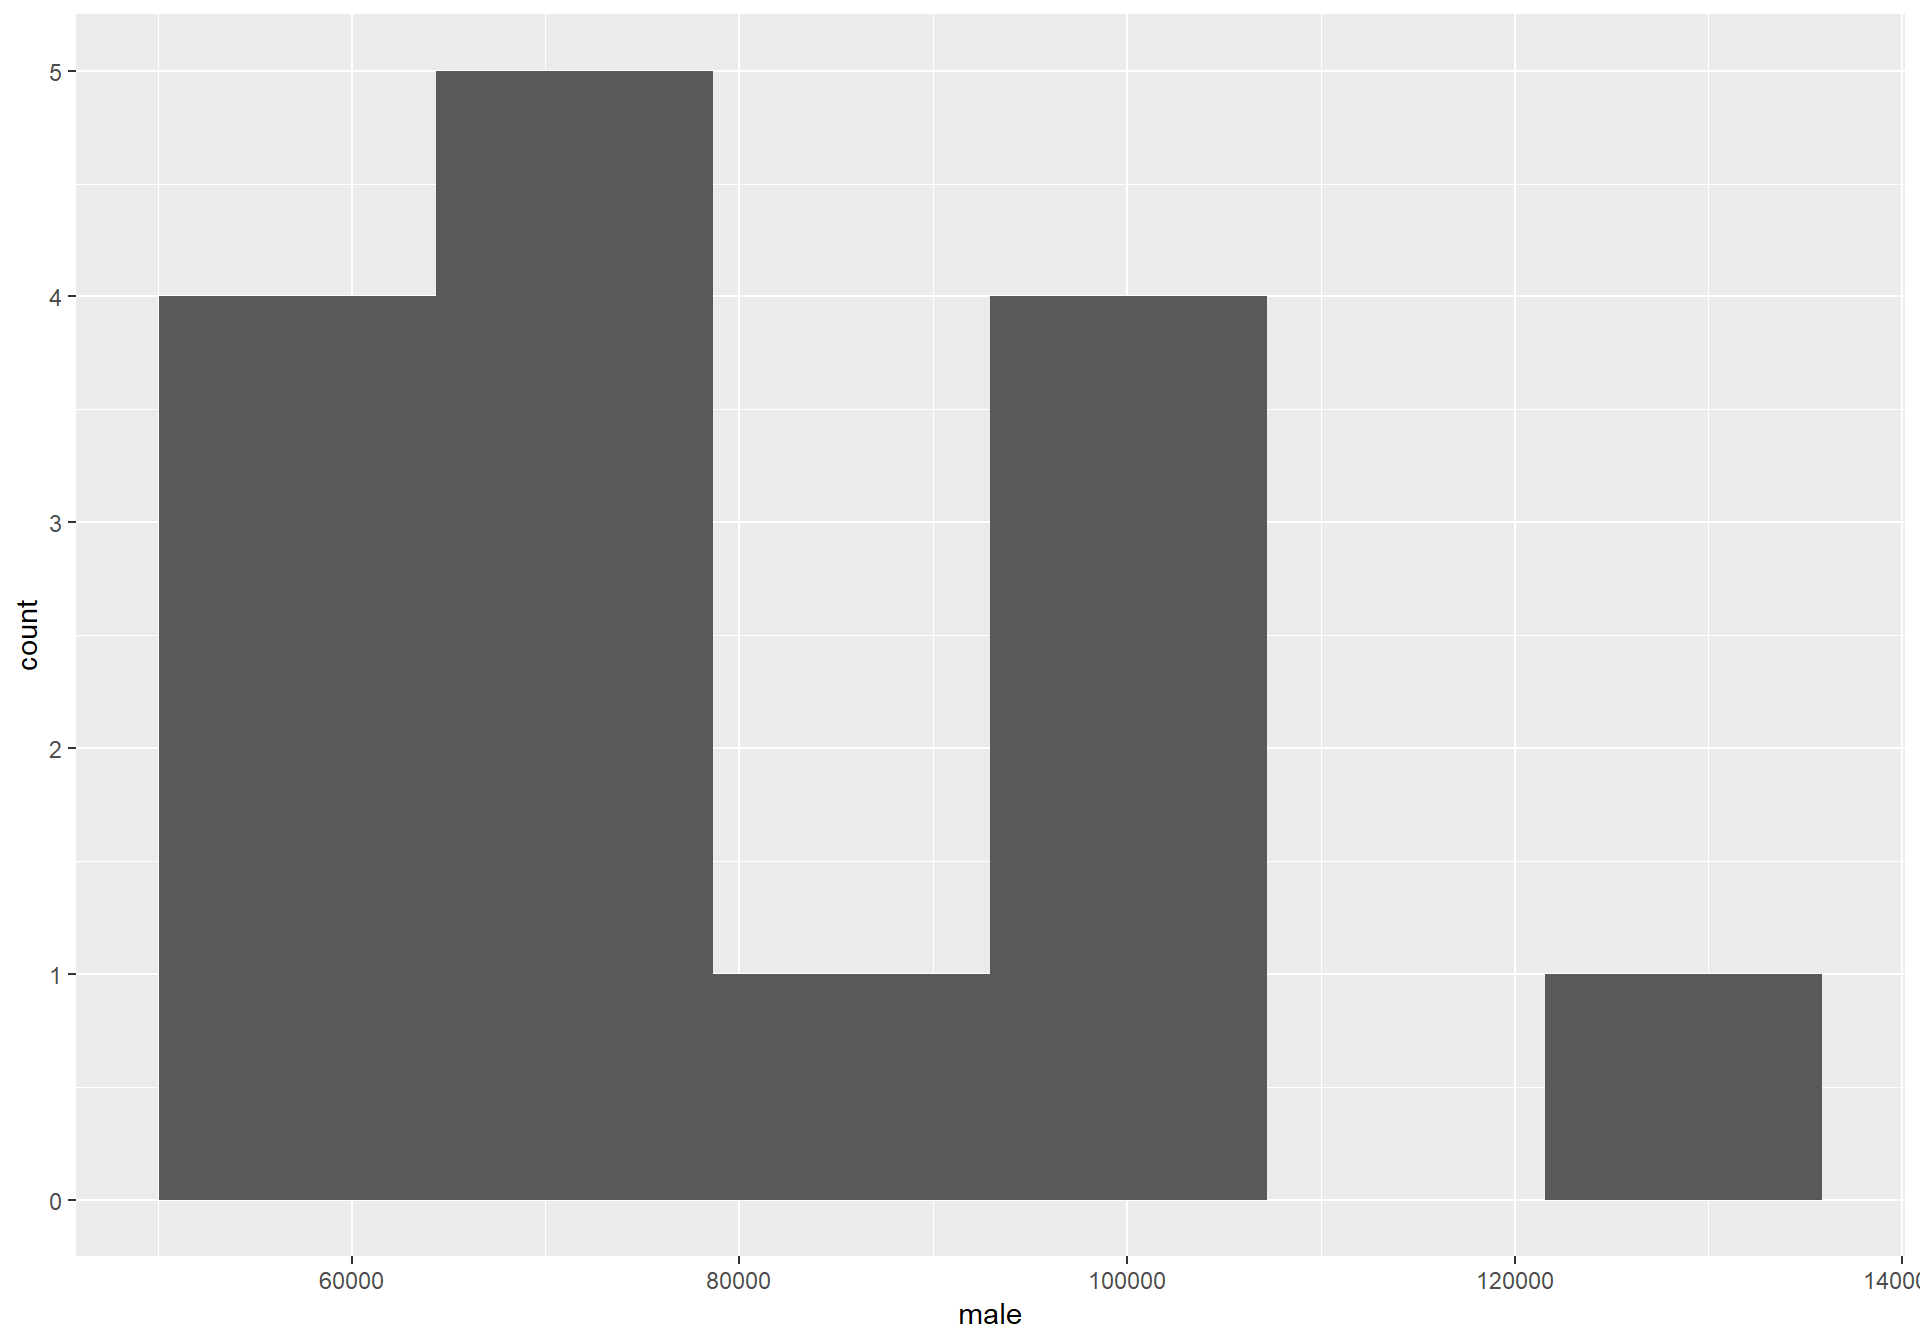
\includegraphics{206_HW_5_files/figure-latex/unnamed-chunk-8-2} \end{center}

\begin{verbatim}
## Warning: Ignoring unknown parameters: stat
\end{verbatim}

\begin{center}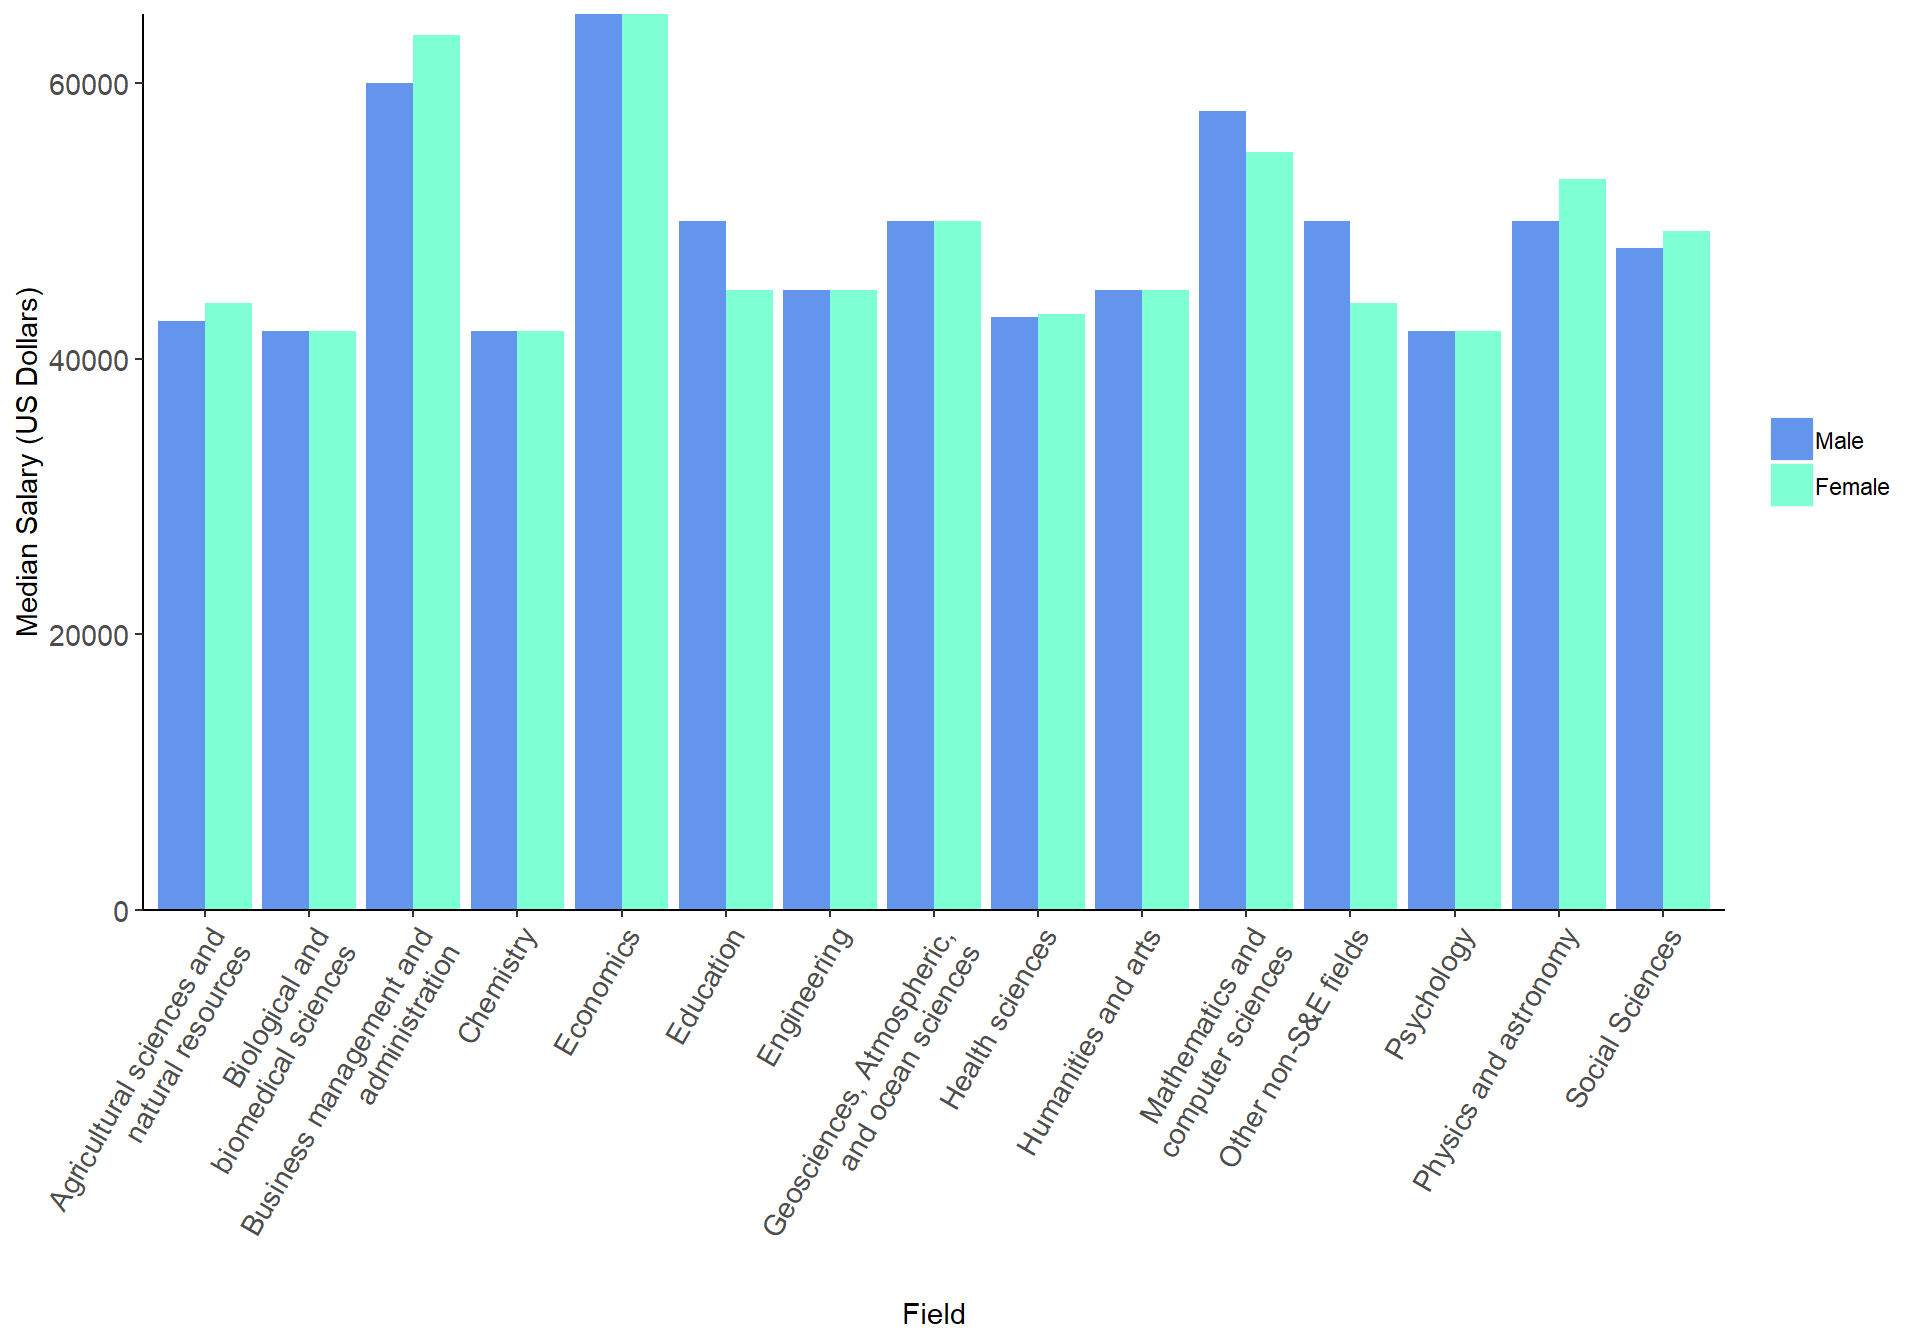
\includegraphics{206_HW_5_files/figure-latex/unnamed-chunk-8-3} \end{center}

\begin{verbatim}
## Warning: Ignoring unknown parameters: stat
\end{verbatim}

\begin{center}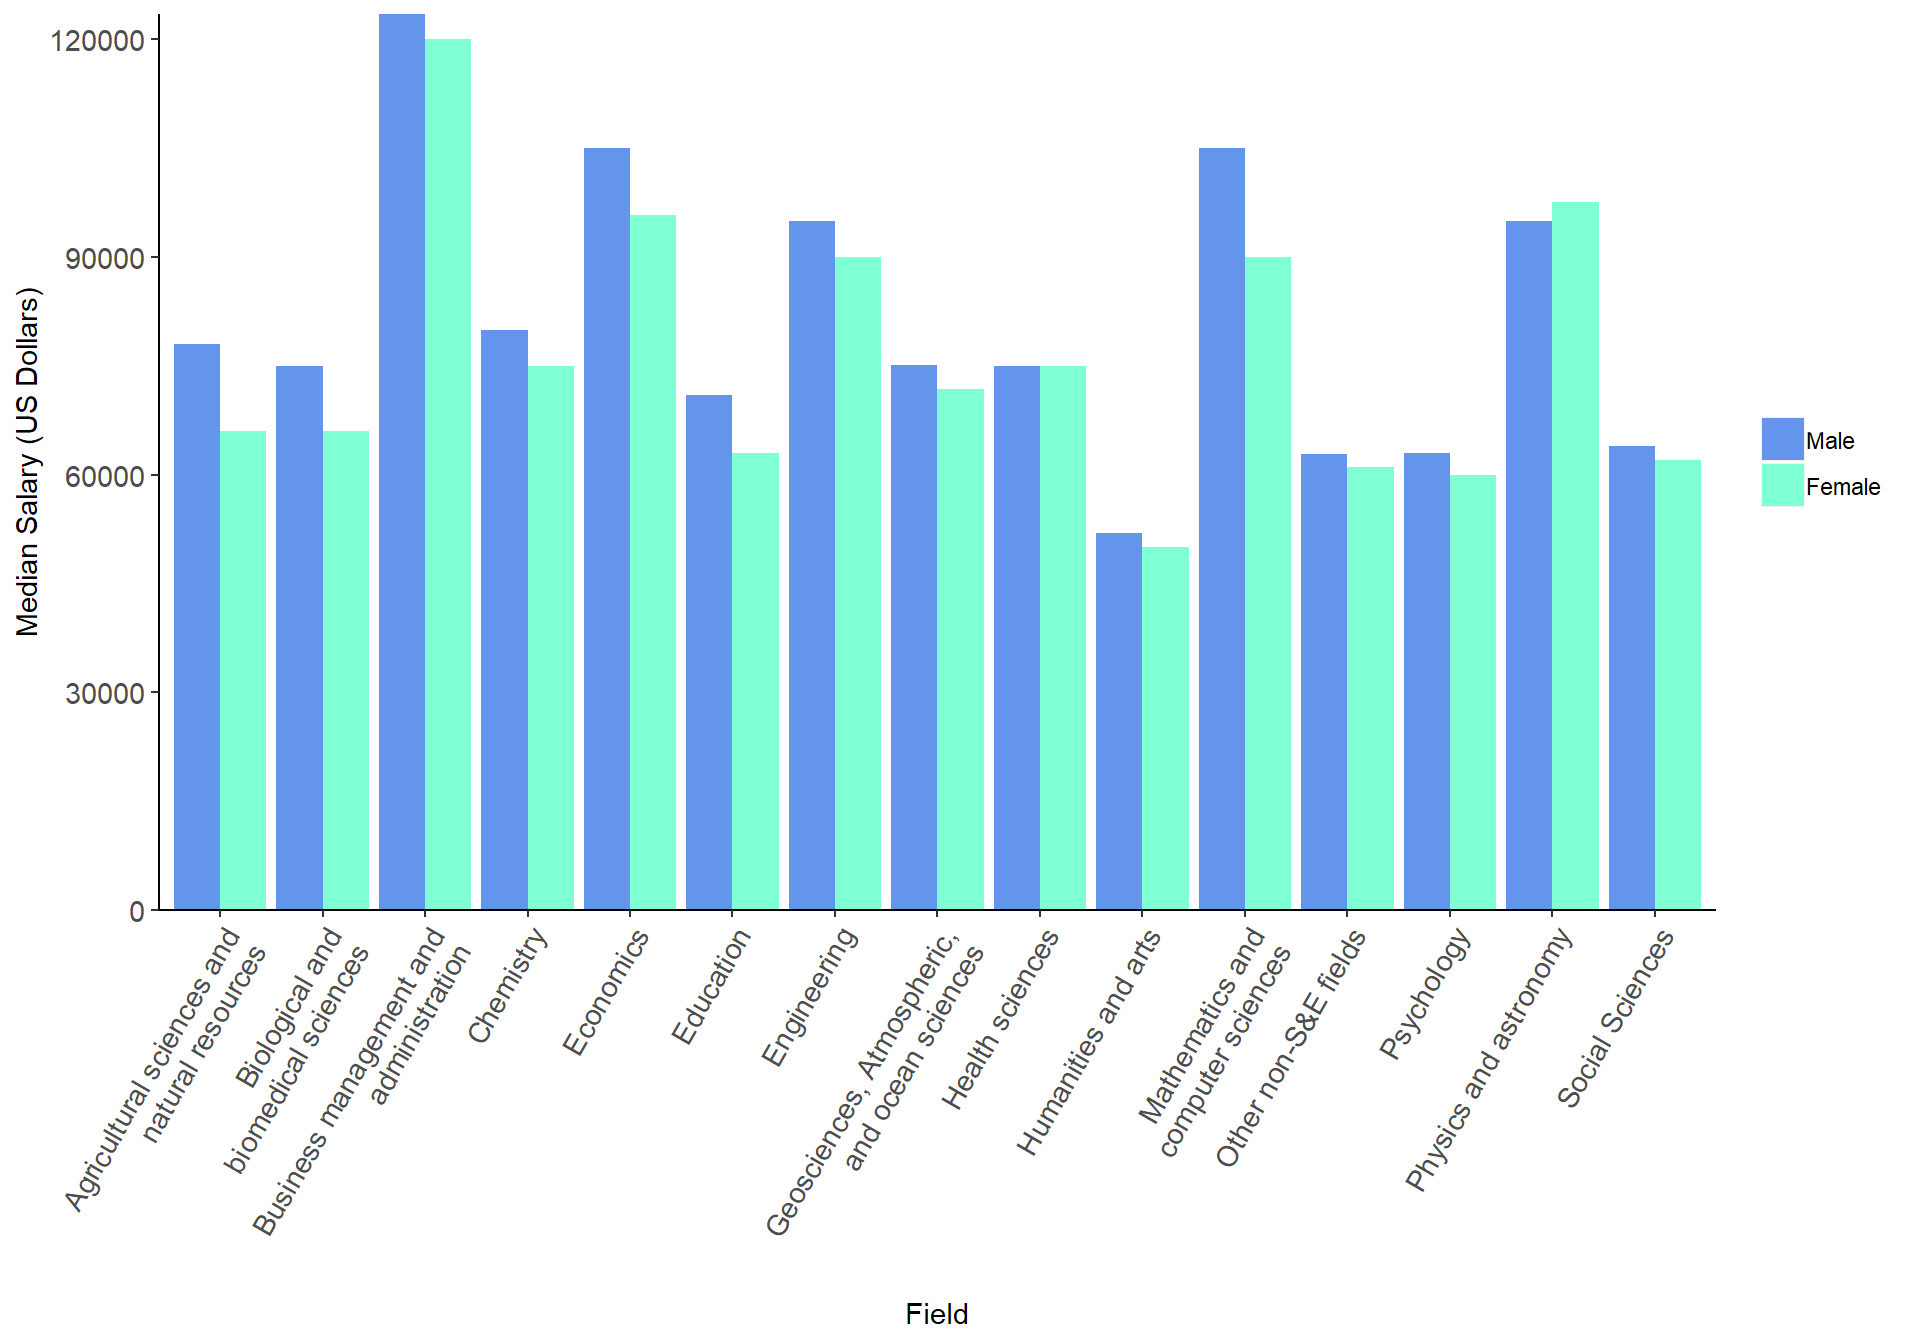
\includegraphics{206_HW_5_files/figure-latex/unnamed-chunk-8-4} \end{center}

There was no significant difference in median salary for male and female
starting postdoc positions (W = 19.5, p = 0.884, alpha = 0.05)

There was a significant difference in median salary for male and female
starting in non-post-doc employment positions (W = 101, p = 0.002, alpha
= 0.05)

\paragraph{4. Exploring academic salaries for professors in U.S.
colleges}\label{exploring-academic-salaries-for-professors-in-u.s.-colleges}

\begin{verbatim}
## 
## Call:
## lm(formula = Salary ~ Faculty_Rank + Years_Since_Phd + Years_Service + 
##     Sex, data = faculty_salary)
## 
## Coefficients:
##          (Intercept)  Faculty_RankAsstProf      Faculty_RankProf  
##              89596.4              -13886.6               33053.4  
##      Years_Since_Phd         Years_Service               SexMale  
##                265.8                -373.8                5499.1
\end{verbatim}

\includegraphics{206_HW_5_files/figure-latex/unnamed-chunk-10-1.pdf}
\includegraphics{206_HW_5_files/figure-latex/unnamed-chunk-10-2.pdf}
\includegraphics{206_HW_5_files/figure-latex/unnamed-chunk-10-3.pdf}
\includegraphics{206_HW_5_files/figure-latex/unnamed-chunk-10-4.pdf}

\begin{verbatim}
## 
## Call:
## lm(formula = Salary ~ Faculty_Rank + Years_Since_Phd + Years_Service + 
##     Sex, data = faculty_salary)
## 
## Residuals:
##    Min     1Q Median     3Q    Max 
## -64844 -14939  -1401  12137 107498 
## 
## Coefficients:
##                      Estimate Std. Error t value Pr(>|t|)    
## (Intercept)           89596.4     4891.1  18.318  < 2e-16 ***
## Faculty_RankAsstProf -13886.6     4333.1  -3.205  0.00146 ** 
## Faculty_RankProf      33053.4     3700.7   8.932  < 2e-16 ***
## Years_Since_Phd         265.8      247.9   1.072  0.28423    
## Years_Service          -373.8      220.8  -1.693  0.09132 .  
## SexMale                5499.1     4034.7   1.363  0.17368    
## ---
## Signif. codes:  0 '***' 0.001 '**' 0.01 '*' 0.05 '.' 0.1 ' ' 1
## 
## Residual standard error: 23580 on 391 degrees of freedom
## Multiple R-squared:  0.4017, Adjusted R-squared:  0.3941 
## F-statistic: 52.51 on 5 and 391 DF,  p-value: < 2.2e-16
\end{verbatim}

\begin{verbatim}
##                     GVIF Df GVIF^(1/(2*Df))
## Faculty_Rank    2.002583  2        1.189591
## Years_Since_Phd 7.271171  1        2.696511
## Years_Service   5.876405  1        2.424130
## Sex             1.029868  1        1.014824
\end{verbatim}

\begin{verbatim}
## [1] 9128.617
\end{verbatim}

\begin{verbatim}
## 
## Call:
## lm(formula = Salary ~ Faculty_Rank + Years_Since_Phd + Sex, data = faculty_salary)
## 
## Coefficients:
##          (Intercept)  Faculty_RankAsstProf      Faculty_RankProf  
##              90957.3              -14012.8               33623.1  
##      Years_Since_Phd               SexMale  
##                -92.1                5146.6
\end{verbatim}

\includegraphics{206_HW_5_files/figure-latex/unnamed-chunk-10-5.pdf}
\includegraphics{206_HW_5_files/figure-latex/unnamed-chunk-10-6.pdf}
\includegraphics{206_HW_5_files/figure-latex/unnamed-chunk-10-7.pdf}
\includegraphics{206_HW_5_files/figure-latex/unnamed-chunk-10-8.pdf}

\begin{verbatim}
## 
## Call:
## lm(formula = Salary ~ Faculty_Rank + Years_Since_Phd + Sex, data = faculty_salary)
## 
## Residuals:
##    Min     1Q Median     3Q    Max 
## -67230 -15338  -1530  12163 105318 
## 
## Coefficients:
##                      Estimate Std. Error t value Pr(>|t|)    
## (Intercept)           90957.3     4836.0  18.808  < 2e-16 ***
## Faculty_RankAsstProf -14012.8     4342.8  -3.227  0.00136 ** 
## Faculty_RankProf      33623.1     3694.1   9.102  < 2e-16 ***
## Years_Since_Phd         -92.1      129.7  -0.710  0.47801    
## SexMale                5146.6     4038.9   1.274  0.20332    
## ---
## Signif. codes:  0 '***' 0.001 '**' 0.01 '*' 0.05 '.' 0.1 ' ' 1
## 
## Residual standard error: 23630 on 392 degrees of freedom
## Multiple R-squared:  0.3973, Adjusted R-squared:  0.3912 
## F-statistic: 64.61 on 4 and 392 DF,  p-value: < 2.2e-16
\end{verbatim}

\begin{verbatim}
##                     GVIF Df GVIF^(1/(2*Df))
## Faculty_Rank    1.979087  2        1.186086
## Years_Since_Phd 1.980427  1        1.407276
## Sex             1.027125  1        1.013472
\end{verbatim}

\begin{verbatim}
## [1] 9129.515
\end{verbatim}

\begin{verbatim}
## 
## Call:
## lm(formula = Salary ~ Faculty_Rank + Years_Service + Sex, data = faculty_salary)
## 
## Coefficients:
##          (Intercept)  Faculty_RankAsstProf      Faculty_RankProf  
##              91315.7              -14702.9               34277.4  
##        Years_Service               SexMale  
##               -171.8                5468.7
\end{verbatim}

\begin{verbatim}
## 
## Call:
## lm(formula = Salary ~ Years_Since_Phd + Sex, data = faculty_salary)
## 
## Coefficients:
##     (Intercept)  Years_Since_Phd          SexMale  
##         85181.8            958.1           7923.6
\end{verbatim}

\begin{verbatim}
## 
## <table style="text-align:center"><tr><td colspan="3" style="border-bottom: 1px solid black"></td></tr><tr><td style="text-align:left"></td><td colspan="2"><em>Dependent variable:</em></td></tr>
## <tr><td></td><td colspan="2" style="border-bottom: 1px solid black"></td></tr>
## <tr><td style="text-align:left"></td><td colspan="2">Salary</td></tr>
## <tr><td style="text-align:left"></td><td>(1)</td><td>(2)</td></tr>
## <tr><td colspan="3" style="border-bottom: 1px solid black"></td></tr><tr><td style="text-align:left">Years_Since_Phd</td><td>958.079<sup>***</sup></td><td></td></tr>
## <tr><td style="text-align:left"></td><td>(108.319)</td><td></td></tr>
## <tr><td style="text-align:left"></td><td></td><td></td></tr>
## <tr><td style="text-align:left">Faculty_RankAsstProf</td><td></td><td>-14,702.860<sup>***</sup></td></tr>
## <tr><td style="text-align:left"></td><td></td><td>(4,266.556)</td></tr>
## <tr><td style="text-align:left"></td><td></td><td></td></tr>
## <tr><td style="text-align:left">Faculty_RankProf</td><td></td><td>34,277.370<sup>***</sup></td></tr>
## <tr><td style="text-align:left"></td><td></td><td>(3,520.957)</td></tr>
## <tr><td style="text-align:left"></td><td></td><td></td></tr>
## <tr><td style="text-align:left">Years_Service</td><td></td><td>-171.792</td></tr>
## <tr><td style="text-align:left"></td><td></td><td>(115.271)</td></tr>
## <tr><td style="text-align:left"></td><td></td><td></td></tr>
## <tr><td style="text-align:left">SexMale</td><td>7,923.624<sup>*</sup></td><td>5,468.708</td></tr>
## <tr><td style="text-align:left"></td><td>(4,684.081)</td><td>(4,035.337)</td></tr>
## <tr><td style="text-align:left"></td><td></td><td></td></tr>
## <tr><td style="text-align:left">Constant</td><td>85,181.820<sup>***</sup></td><td>91,315.670<sup>***</sup></td></tr>
## <tr><td style="text-align:left"></td><td>(4,748.315)</td><td>(4,621.700)</td></tr>
## <tr><td style="text-align:left"></td><td></td><td></td></tr>
## <tr><td colspan="3" style="border-bottom: 1px solid black"></td></tr><tr><td style="text-align:left">Observations</td><td>397</td><td>397</td></tr>
## <tr><td style="text-align:left">R<sup>2</sup></td><td>0.182</td><td>0.400</td></tr>
## <tr><td style="text-align:left">Adjusted R<sup>2</sup></td><td>0.178</td><td>0.394</td></tr>
## <tr><td style="text-align:left">Residual Std. Error</td><td>27,468.940 (df = 394)</td><td>23,581.860 (df = 392)</td></tr>
## <tr><td style="text-align:left">F Statistic</td><td>43.742<sup>***</sup> (df = 2; 394)</td><td>65.324<sup>***</sup> (df = 4; 392)</td></tr>
## <tr><td colspan="3" style="border-bottom: 1px solid black"></td></tr><tr><td style="text-align:left"><em>Note:</em></td><td colspan="2" style="text-align:right"><sup>*</sup>p<0.1; <sup>**</sup>p<0.05; <sup>***</sup>p<0.01</td></tr>
## </table>
\end{verbatim}


\end{document}
